\documentclass[10pt]{beamer}
\usetheme{Madrid}
\usecolortheme{default}
\usefonttheme{professionalfonts}

\usepackage{amsmath,amssymb,bm}
\usepackage{tikz}
\usetikzlibrary{arrows.meta,positioning}
\usepackage{booktabs}
\usepackage{xcolor}
\usepackage{appendixnumberbeamer}   % keeps appendix out of total frame count

\setbeamertemplate{navigation symbols}{}
\setbeamerfont{frametitle}{size=\normalsize,series=\bfseries}

% ── Section-progress slider in the headline ───────────────────────────────────
\setbeamertemplate{headline}{%
  \leavevmode%
  \begin{beamercolorbox}[wd=\paperwidth,ht=2.5ex,dp=1.25ex]{section in head/foot}%
    \insertsectionnavigationhorizontal{\paperwidth}{\hskip0.6em}{\hskip0.6em}%
  \end{beamercolorbox}%
}

\title[$\rho$-GNF Sensitivity Analysis]{%
  Sensitivity Analysis for Unobserved Confounding\\%
  via $\rho$-Graphical Normalizing Flows}
\author{Matej Havelka}
\institute{WI4050}
\date{June 2026}

\begin{document}

% ─────────────────────────────────────────────────────────────────────────────
\begin{frame}
  \titlepage
\end{frame}

% =============================================================================
\section{Causal Inference}
% =============================================================================

% ── 1. Does Smoking Cause Lung Cancer? ───────────────────────────────────────
\begin{frame}{Does Smoking Cause Lung Cancer?}
  \begin{center}
  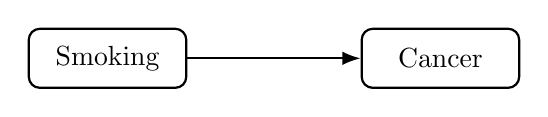
\begin{tikzpicture}[
    node distance=2.2cm,
    box/.style={rectangle,draw,thick,rounded corners,minimum width=2.0cm,
                minimum height=0.75cm,font=\normalsize},
    >=Latex,thick
  ]
    \node[box] (S) {Smoking};
    \node[box,right=of S] (C) {Cancer};
    \draw[->] (S) -- (C);
  \end{tikzpicture}
  \end{center}
  \bigskip
  \begin{center}
    \large\itshape
    Smokers have higher cancer rates.\\[6pt]
    Is this arrow real?
  \end{center}
\end{frame}

% ── 2. Unobserved Confounding ─────────────────────────────────────────────────
\begin{frame}{Or Do Smokers Just Live Differently?}
  \begin{center}
  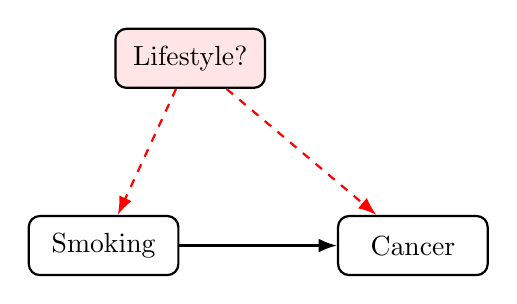
\begin{tikzpicture}[
    node distance=1.6cm and 2.0cm,
    box/.style={rectangle,draw,thick,rounded corners,minimum width=1.9cm,
                minimum height=0.75cm,font=\normalsize},
    >=Latex,thick
  ]
    \node[box] (S) {Smoking};
    \node[box,right=of S] (C) {Cancer};
    \node[box,above=of S,xshift=1.1cm,fill=red!10] (U) {Lifestyle?};
    \draw[->] (S) -- (C);
    \draw[->,dashed,red,thick] (U) -- (S);
    \draw[->,dashed,red,thick] (U) -- (C);
  \end{tikzpicture}
  \end{center}
  \bigskip
  \begin{center}
    \large\itshape
    What if heavy smokers also drink more,\\
    exercise less, eat differently, \ldots?
  \end{center}
\end{frame}

% ── 3. Conditional Ignorability ───────────────────────────────────────────────
\begin{frame}{What If We Could Measure Everything?}
  \begin{center}
  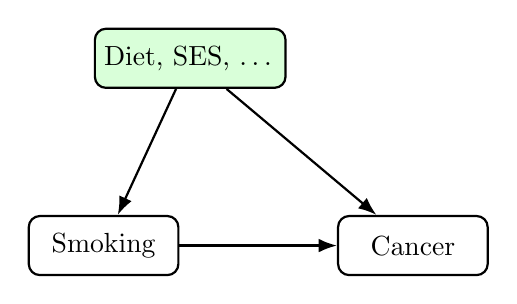
\begin{tikzpicture}[
    node distance=1.6cm and 2.0cm,
    box/.style={rectangle,draw,thick,rounded corners,minimum width=1.9cm,
                minimum height=0.75cm,font=\normalsize},
    >=Latex,thick
  ]
    \node[box] (S) {Smoking};
    \node[box,right=of S] (C) {Cancer};
    \node[box,above=of S,xshift=1.1cm,fill=green!15] (X) {Diet, SES, \ldots};
    \draw[->] (S) -- (C);
    \draw[->,thick] (X) -- (S);
    \draw[->,thick] (X) -- (C);
  \end{tikzpicture}
  \end{center}
  \begin{center}
    \large\itshape
    Observe all confounders $X$\,:
  \end{center}
  \[
    Y(a) \;\perp\!\!\!\perp\; A \;\big|\; X
    \qquad \Longrightarrow \qquad
    \mathbb{E}[Y \mid \mathrm{do}(A{=}a)]
    = \mathbb{E}_X\!\bigl[\mathbb{E}[Y \mid A=a,X]\bigr]
  \]
\end{frame}

% ── 4. ATE + Sensitivity Motivation ──────────────────────────────────────────
\begin{frame}{What Do We Actually Want to Measure?}
  \[
    \tau \;=\;
    \mathbb{E}\bigl[Y \mid \mathrm{do}(A=1)\bigr]
    -
    \mathbb{E}\bigl[Y \mid \mathrm{do}(A=0)\bigr]
  \]
  \begin{center}\itshape
    But $U$ is unobserved — ignorability fails.\\[6pt]
    How sensitive is $\hat\tau$ to the strength of $U$?
  \end{center}
  \medskip
  \begin{enumerate}
    \item Fix scalar confounding strength $\rho$
    \item Estimate $\hat\tau(\rho)$
    \item Report full $\rho$-curve; let domain knowledge bound $\rho$
  \end{enumerate}
\end{frame}

% =============================================================================
\section{$\rho$-GNF Model}
% =============================================================================

% ── 5. Gaussian Copula as ρ ───────────────────────────────────────────────────
\begin{frame}{Gaussian Copula as Sensitivity Parameter}
  \textit{Unobserved confounding $\equiv$ latent Gaussian correlation $\rho$.}
  \[
    C_\rho(u,v) \;=\; \Phi_\rho\!\bigl(\Phi^{-1}(u),\;\Phi^{-1}(v)\bigr)
  \]
  \[
    (z_A,\; z_Y) \;\sim\; \mathcal{N}\!\left(\mathbf{0},\;
    \Sigma_\rho = \begin{pmatrix}1 & \rho \\ \rho & 1\end{pmatrix}\right)
  \]
  \[
    \rho = 0: \text{ no confounding} \qquad |\rho| \to 1: \text{ maximal}
  \]
\end{frame}

% ── 6. ρ-GNF Generative Model ─────────────────────────────────────────────────
\begin{frame}{$\rho$-GNF: Generative Model}
  \textit{Correlated latents flow through a learned causal bijection $f_\theta$.}
  \begin{columns}[c]
    \column{0.46\textwidth}
    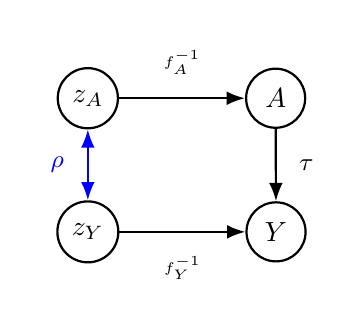
\begin{tikzpicture}[
      node distance=0.9cm and 1.5cm,
      every node/.style={circle,draw,thick,minimum size=0.75cm,font=\normalsize},
      >=Latex,thick
    ]
      \node (zA) {$z_A$};
      \node[below=0.9cm of zA] (zY) {$z_Y$};
      \node[right=1.6cm of zA] (A) {$A$};
      \node[right=1.6cm of zY] (Y) {$Y$};
      \draw[<->,blue,thick] (zA) -- (zY)
            node[midway,left,draw=none,blue,font=\small] {$\rho$};
      \draw[->] (zA) -- (A)
            node[midway,above,draw=none,font=\tiny] {$f_A^{-1}$};
      \draw[->] (zY) -- (Y)
            node[midway,below,draw=none,font=\tiny] {$f_Y^{-1}$};
      \draw[->] (A) -- (Y)
            node[midway,right,draw=none,font=\small] {$\tau$};
    \end{tikzpicture}
    \column{0.54\textwidth}
    \[
      p(A,Y) \;=\; p_Z\!\bigl(f(A,Y)\bigr)\,\bigl|\det J_f\bigr|
    \]
    \smallskip
    $f_\theta$ learned end-to-end via max.\ likelihood\\[4pt]
    \textcolor{gray}{\small(architecture details: backup slides)}
  \end{columns}
\end{frame}

% ── 7. ATE Estimator ─────────────────────────────────────────────────────────
\begin{frame}{ATE Estimator via Flow Inversion}
  \textit{Pin $z_A$; invert; read off $Y$. Average over noise draws.}
  \[
    \hat\tau
    \;=\; \frac{1}{S}\sum_{s=1}^{S}
    \Bigl[
      \bigl[f^{-1}(\mathbf{z}^{(s)},\; z_A{=}1)\bigr]_Y
      \;-\;
      \bigl[f^{-1}(\mathbf{z}^{(s)},\; z_A{=}0)\bigr]_Y
    \Bigr]
  \]
  \[
    (z_A^{(s)},\; z_Y^{(s)}) \;\sim\; \mathcal{N}(\mathbf{0},\;\Sigma_\rho)
  \]
  Do-intervention in latent space; propagated through $f^{-1}$.
\end{frame}

% =============================================================================
\section{Experiments}
% =============================================================================

% ── 8. Setting 0: DGP ────────────────────────────────────────────────────────
\begin{frame}{Setting 0: Gaussian DGP (Sanity Check)}
  \textit{Model is correctly specified. Does it recover $\rho^*$?}
  \[
    \begin{pmatrix}e_A \\ e_Y\end{pmatrix}
    \sim \mathcal{N}\!\left(\mathbf{0},\;
    \begin{pmatrix}1 & \rho^* \\ \rho^* & 1\end{pmatrix}\right)
    ,\quad A = e_A,\quad Y = 0.2\, A + e_Y
  \]
  \[
    \rho^* = 0.30,\qquad \text{True ATE} = 0.20
  \]
\end{frame}

% ── 9. Setting 0: Results ─────────────────────────────────────────────────────
\begin{frame}{Setting 0: Results}
  \textit{Minimum RMSE at assumed $\rho \approx \rho^*$. Model is identifiable.}
  \begin{center}
  \renewcommand{\arraystretch}{1.25}
  \begin{tabular}{rcc}
    \toprule
    Assumed $\rho$ & Mean $\hat\tau$ & RMSE \\
    \midrule
    $0.156$ & $0.343$ & $0.149$ \\
    $\mathbf{0.261}$ & $\mathbf{0.228}$ & $\mathbf{0.044}$ \\
    $0.365$ & $0.109$ & $0.096$ \\
    \bottomrule
  \end{tabular}
  \end{center}
  \medskip
  $n = 5000$, $5$ seeds. True ATE $= 0.20$,\; $\rho^* = 0.30$.
\end{frame}

% ── 10. Setting 1: Clayton DGP ────────────────────────────────────────────────
\begin{frame}{Setting 1: Clayton Copula (Misspecification)}
  \textit{True copula has lower-tail dependence; Gaussian model is wrong.}
  \[
    C_\theta(u,v) \;=\; \bigl(u^{-\theta}+v^{-\theta}-1\bigr)^{-1/\theta},
    \qquad \lambda_L = 2^{-1/\theta}
  \]
  \[
    \tau_K = \frac{\theta}{\theta+2}\;,
    \qquad
    \rho_{\mathrm{ref}} = \sin\!\left(\frac{\pi\,\tau_K}{2}\right)
    \approx 0.707 \quad(\theta = 2)
  \]
\end{frame}

% ── 11. Setting 1: Results ────────────────────────────────────────────────────
\begin{frame}{Setting 1: Results}
  \textit{Copula mismatch shifts optimal $\rho$ and inflates RMSE.}
  \begin{center}
  \renewcommand{\arraystretch}{1.25}
  \begin{tabular}{rcc}
    \toprule
    Assumed $\rho$ & Mean $\hat\tau$ & RMSE \\
    \midrule
    $\rho_{\mathrm{ref}} = 0.707$ & $-0.038$ & $0.240$ \\
    $\bm{\rho_{\mathrm{opt}} = 0.550}$ & $\mathbf{0.216}$ & $\mathbf{0.053}$ \\
    \bottomrule
  \end{tabular}
  \end{center}
  \medskip
  RMSE at $\rho_{\mathrm{ref}}$ is $\mathbf{4.5\times}$ higher than at $\rho_{\mathrm{opt}}$.
  True ATE $= 0.20$.
\end{frame}

% =============================================================================
\section{Limitations}
% =============================================================================

% ── 12. Limitation 1: Gaussian Copula Assumption ─────────────────────────────
\begin{frame}{Limitation 1: Gaussian Copula Is a Strong Assumption}
  \textit{All confounding is forced into a Gaussian shape — regardless of reality.}
  \[
    (z_A,z_Y)\sim\mathcal{N}(\mathbf{0},\Sigma_\rho)
    \quad\text{for \emph{every} dataset, \emph{every} DGP}
  \]
  \begin{itemize}
    \item Clayton tail dependence $\neq$ Gaussian tail dependence
    \item Optimal $\rho$ shifts away from the Kendall-matched $\rho_{\mathrm{ref}}$
    \item Model \emph{compensates} with a wrong $\rho$, not a correct copula
  \end{itemize}
\end{frame}

% ── 13. Limitation 2: ρ Cannot Depend on Observed Covariates ─────────────────
\begin{frame}{Limitation 2: $\rho$ Is Blind to Observed Covariates}
  \textit{$\rho$ is one global constant — it cannot vary with $X$.}
  \begin{columns}[c]
    \column{0.5\textwidth}
    \[
      (z_A,z_Y)\sim\mathcal{N}(\mathbf{0},\Sigma_{\textcolor{red}{\rho}})
    \]
    Same $\rho$ for all observations,\\
    even when confounding strength\\
    clearly varies across subgroups.
    \column{0.5\textwidth}
    \textbf{Example:} Clayton $\theta(X) = 0.5 + 3.5\,X$
    \[
      X\!\to\!0:\;\text{weak confounding}
    \]
    \[
      X\!\to\!1:\;\text{strong confounding}
    \]
    Original $\rho$-GNF has no mechanism\\
    to use $X$ when estimating $\hat\tau$.
  \end{columns}
\end{frame}

% =============================================================================
\section{Extension}
% =============================================================================

% ── 14. Extension: Context Conditioning ──────────────────────────────────────
\begin{frame}{Extension: Context Conditioning}
  \textit{DGP: $\theta(X) \in [0.5,\,4]$ with $X \sim U[0,1]$. Can the model adapt?}
  \begin{columns}[c]
    \column{0.48\textwidth}
    \textbf{V1} — fixed $\rho$, no context:
    \[
      h_i = \mathrm{MLP}(e_i)
    \]

    \textbf{V2} — condition on $X$:
    \[
      h_i = \mathrm{MLP}(e_i \;\|\; X)
    \]

    \column{0.52\textwidth}
    \begin{center}
    \fbox{%
      \parbox{3.6cm}{\centering
        \vspace{1.0cm}
        {\small\itshape Setting 2 results\\[4pt]pending}
        \vspace{1.0cm}
      }%
    }
    \end{center}
  \end{columns}
\end{frame}

% ── Q&A ──────────────────────────────────────────────────────────────────────
\begin{frame}
  \begin{center}
    \vspace{1.5cm}
    {\Huge Thank you}\\[1.5cm]
    {\Large Questions?}
  \end{center}
\end{frame}

% =============================================================================
% BACKUP SLIDES (not counted in total; shown only if questions arise)
% =============================================================================
\appendix

\begin{frame}{Backup: DAGConditioner — Encoding Causal Order}
  \textit{Mask $M$ ensures $h_i$ sees only causal parents.}
  \[
    h_i \;=\; \mathrm{MLP}\!\bigl(M_{i,:} \odot x\bigr),
    \qquad M_{ij} = \mathbf{1}\bigl[j \in \mathrm{pa}(i)\bigr]
  \]
  For the graph $A \to Y$:
  \[
    h_A = \mathrm{MLP}(\mathbf{0}),
    \qquad
    h_Y = \mathrm{MLP}(A)
  \]
  Adjacency $A_\theta$ trained via Gumbel-softmax; $\ell_1$ sparsity.
\end{frame}

\begin{frame}{Backup: UMNN — Unconstrained Monotone Neural Network}
  \textit{Each variable maps through a strictly monotone bijection.}
  \[
    z_i \;=\; \int_0^{x_i} g_\phi\!\bigl(t;\; h_i\bigr)\;\mathrm{d}t \;+\; b_i,
    \qquad g_\phi > 0
  \]
  \[
    \log\left|\frac{\partial z_i}{\partial x_i}\right|
    \;=\; \log g_\phi(x_i;\; h_i)
  \]
  $g_\phi$: MLP $+$ \texttt{softplus}. Jacobian is exact, not approximated.
\end{frame}

\begin{frame}{Backup: Training Objective}
  \textit{Maximize log-likelihood; $\Sigma_\rho$ fixed.}
  \[
    \mathcal{L}(\theta)
    \;=\; \frac{1}{N}\sum_{n=1}^N
    \Bigl[
      \log p_Z\!\bigl(z^{(n)}\bigr)
      \;+\;
      \log\bigl|\det J_f(x^{(n)})\bigr|
    \Bigr]
  \]
  \[
    p_Z(z) \;=\; \mathcal{N}(z;\;\mathbf{0},\;\Sigma_\rho)
  \]
  Only the flow parameters $\theta$ are optimized; $\rho$ is a hyperparameter.
\end{frame}

\end{document}
